\documentclass{article}%
\usepackage[T1]{fontenc}%
\usepackage[utf8]{inputenc}%
\usepackage{lmodern}%
\usepackage{textcomp}%
\usepackage{lastpage}%
\usepackage{geometry}%
\geometry{a4paper, left=15mm, right=15mm, top=15mm, bottom=15mm}%
\usepackage{xcolor}%
\usepackage{longtable}%
\usepackage{graphicx}%
\usepackage{titlesec}%
\usepackage{datetime}%
\usepackage{extramarks}%
\usepackage{fancyhdr}%
\pagestyle{fancy}%
\fancyhf{}%
\lhead{MOLECULAR CALCULATION REPORT}%
\rhead{Generated by quchemreport}%
\lfoot{\today ~  \currenttime}%
\rfoot{Page \thepage}%
\cfoot{}%
\renewcommand\headrulewidth{0.4pt}%
\renewcommand\footrulewidth{0.4pt}%
\definecolor{ufrblue}{RGB}{0,161,140}%
\definecolor{bordeau}{RGB}{125,31,31}%
\titleformat{name=\section}[block]{\sc\large}{}{0pt}{\colorsection}%
\titlespacing{\section}{0pt}{\baselineskip}{2pt}%
\titlespacing{\subsection}{4pt}{\baselineskip}{0pt}%
\newcommand{\colorsection}[1]{\colorbox{ufrblue}{\parbox{\dimexpr\textwidth-2\fboxsep}{\textcolor{white}{\textbf{{\thesection.\ #1}}}}}}%
\usepackage{tabularx}%
\usepackage{longtable}%
%
%
%
\begin{document}%
\small%
\section{MOLECULE}%
\label{sec:MOLECULE}%
\begin{figure}[h]%
\begin{center}%
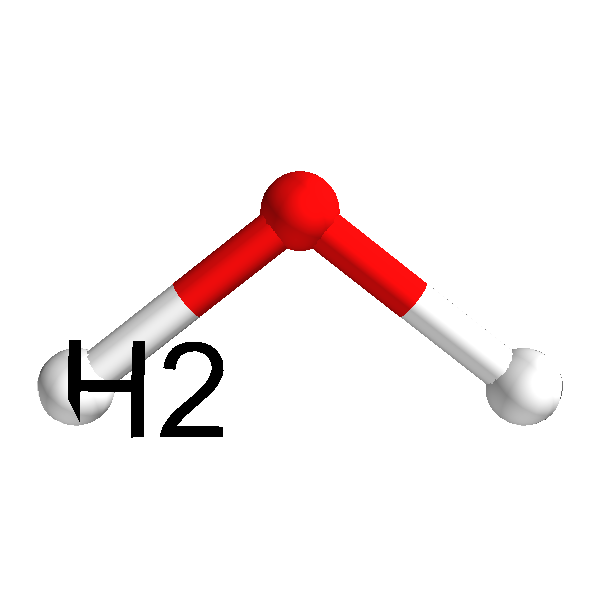
\includegraphics[width=7cm]{temp/img-TOPOLOGY.png}%
\includegraphics[width=7cm]{temp/img-TOPOLOGY_cam2.png}%
\end{center}%
\vspace{-5mm}%
\caption{Chemical structure diagram with atomic numbering from two points of view.}%
\end{figure}%
\begin{tabularx}{\textwidth}{|l X|}%
Directory name&QuChem\\%
Formula&H2O\\%
Charge&0\\%
Spin multiplicity&1\\%
Monoisotopic mass&18.01056 Da\\%
InChI&1S/H2O/h1H2\\%
SMILES&O\\%
\end{tabularx}

%
\section{COMPUTATIONAL DETAILS}%
\label{sec:COMPUTATIONALDETAILS}%
\begin{tabularx}{\textwidth}{|l X| X|}%
Software&Gaussian&(2009+D.01)\\%
Computational method&DFT& \\%
Functional&B3LYP& \\%
Basis set name&6{-}31G(d)& \\%
Number of basis set functions&19& \\%
Closed shell calculation&True& \\%
Requested SCF convergence on RMS and Max density matrix&1e{-}08&1e{-}06\\%
Requested SCF convergence on energy&1e{-}06& \\%
Job type: Time{-}dependent calculation& & \\%
Number of calculated excited states and spin state&5&{[}'Singlet{-}A1' 'Singlet{-}A2' 'Singlet{-}B1' 'Singlet{-}B2'{]}\\%
 & & \\%
 & & \\%
Job type: Geometry optimization& & \\%
Max Force value and threshold&0.000156&0.000450\\%
RMS Force value and threshold&0.000101&0.000300\\%
Max Displacement value and threshold&0.000578&0.001800\\%
RMS Displacement value and threshold&0.000550&0.001200\\%
 & & \\%
\end{tabularx}

%
\section{RESULTS}%
\label{sec:RESULTS}%
\begin{tabularx}{\textwidth}{|l X| X|}%
Total molecular energy&{-}76.40895 hartrees& \\%
HOMO number&5& \\%
LUMO+1 energies&4.03 eV& \\%
LUMO   energies&1.70 eV& \\%
HOMO   energies&{-}7.92 eV& \\%
HOMO{-}1 energies&{-}10.13 eV& \\%
 & & \\%
 & & \\%
Geometry optimization specific results& & \\%
Converged nuclear repulsion energy&9.08784 Hartrees& \\%
 & & \\%
Mean Mulliken atomic charge and standard deviation&0.0000 e{-}&0.5475 e{-}\\%
Atoms with negatives charges under the standard deviation&N°&Mulliken charge\\%
 &O 1&  {-}0.774\\%
Atoms with positives charges over the standard deviation&N°&Mulliken charge\\%
\end{tabularx}%
\begin{figure}[h]%
\begin{center}%
\includegraphics[width=7cm]{temp/img-MO-homo.png}%
\includegraphics[width=7cm]{temp/img-MO-homo_cam2.png}%
\end{center}%
\vspace{-5mm}%
\caption{Representation of the HOMO from two points of view.}%
\end{figure}%
\begin{figure}[h]%
\begin{center}%
\includegraphics[width=7cm]{temp/img-MO-lumo.png}%
\includegraphics[width=7cm]{temp/img-MO-lumo_cam2.png}%
\end{center}%
\vspace{-5mm}%
\caption{Representation of the LUMO from two points of view.}%
\end{figure}%
\begin{center}%
\begin{tabular}{rrrrrrrrrp{6cm}}%
\multicolumn{10}{c}{Table. Results concerning the calculated mono{-}electronic excitations.}\\%
E.S.&Symmetry& nm &cm$^{-1}$&\textit{f}&R&$\Lambda$&d$_{CT}$&q$_{CT}$&Excitation description : initial OM {-} ending OM (\% if > 5\%)\\%
\hline%
1&Singlet{-}B1&156 &63850 &0.014&0.0&0.41&88.49&0.82& 5{-}6(100); \\%
2&Singlet{-}A2&124 &80171 &0.000&0.0&0.38&80.85&0.82& 5{-}7(99); \\%
3&Singlet{-}A1&118 &84705 &0.095&0.0&0.53&111.71&0.72& 4{-}6(98); \\%
4&Singlet{-}B2&97 &102261 &0.072&0.0&0.53&104.36&0.72& 4{-}7(95); \\%
5&Singlet{-}B2&85 &117079 &0.398&0.0&0.59&76.69&0.68& 3{-}6(95); \\%
\hline%
\end{tabular}%
\end{center}%
\begin{figure}[h]%
\begin{center}%
\includegraphics[width=10cm]{temp/img-UV-Abso-Spectrum.png}%
\end{center}%
\vspace{-5mm}%
\caption{Calculated UV visible Absorption spectrum with a gaussian broadening (FWHM = 3000 cm-1)}%
\end{figure}%
\begin{figure}[h]%
\begin{center}%
\includegraphics[width=10cm]{temp/img-UV-CD-Spectrum.png}%
\end{center}%
\vspace{-5mm}%
\caption{Calculated Circular Dichroism spectrum with a gaussian broadening (FWHM = 3000 cm-1)}%
\end{figure}%
\begin{figure}[h]%
\begin{center}%
\includegraphics[width=7cm]{temp/img-EDD-S1.png}%
\includegraphics[width=7cm]{temp/img-EDD-S1_cam2.png}%
\end{center}%
\vspace{-5mm}%
\caption{Representation of the Electron Density Difference (S1-S0) from two points of view.}%
\end{figure}%
\begin{figure}[h]%
\begin{center}%
\includegraphics[width=7cm]{temp/img-EDD-S2.png}%
\includegraphics[width=7cm]{temp/img-EDD-S2_cam2.png}%
\end{center}%
\vspace{-5mm}%
\caption{Representation of the Electron Density Difference (S2-S0) from two points of view.}%
\end{figure}%
\begin{footnotesize}%
\begin{center}%
\begin{longtable}{p{0.5cm}rrrrp{0.5cm}}%
\multicolumn{6}{c}{Table. Converged cartesian atomic coordinates in Angstroms}\\%
&Atom&\multicolumn{1}{c}{X}&\multicolumn{1}{c}{Y}&\multicolumn{1}{c}{Z}&\\%
\hline%
&O&0.0000&0.0000&0.1198&\\%
&H&0.0000&0.7613&{-}0.4792&\\%
&H&0.0000&{-}0.7613&{-}0.4792&\\%
\hline%
\end{longtable}%
\end{center}%
\end{footnotesize}

%
\end{document}